\chapter{Homogene katalyse in de industrie}\label{ch:b3:homogeneous-catalysis}

Het grootste deel van het azijnzuur ter wereld, de grondstof van
vinylacetaat, van celluloseacetaat en van het gezuiverde tereftaalzuur van
plastic flessen, wordt in enkele zeer grote fabrieken gemaakt uit
methanol en koolstofmonoxide. In elk ervan doorloopt een rodium- of
iridiumcomplex, in lage concentratie opgelost in de reactievloeistof,
duizenden cycli per uur, jarenlang. Hetzelfde soort chemie hydrogeneert,
voegt CO en waterstof toe aan alkenen, wisselt de uiteinden van dubbele
bindingen uit, koppelt aromatische ringen en maakt polyetheen en
polypropeen per miljoen ton. Dit hoofdstuk leest de katalytische cycli
van de belangrijkste industriële processen met de instrumenten van
\cref{ch:b3:organometallic-bonding}: elektronentellingen,
oxidatietoestanden, snelheidsbepalende stappen, en de symmetrie van de
katalysator die de structuur van een polymeer vastlegt.

\begin{recall}
Het deel van jaar~2 voerde de elementaire stappen van
organometaalreacties in (oxidatieve additie, reductieve eliminatie,
migratorische insertie, $\beta$-hydride-eliminatie, transmetallering),
katalytische cycli, prekatalysatoren, turnovergetal en
turnoverfrequentie, en las de cycli van hydrogenering, \omterm{def:b3:homogeneous-catalysis:hydroformylation}{hydroformylering}
en kruiskoppeling; het definieerde ook de tacticiteit en de
ketengroeipolymerisatie, de omzetting en de selectiviteit.
\Cref{ch:b3:organometallic-bonding} telde elektronen en beschreef
carbonyl- en carbeenliganden;
\cref{ch:b3:complex-kinetics} gaf de verzadigingskinetiek;
\cref{ch:b3:point-groups} de \omterm{def:b3:point-groups:operation}{symmetrie-elementen} van moleculen.
\end{recall}

\begin{omfigure}
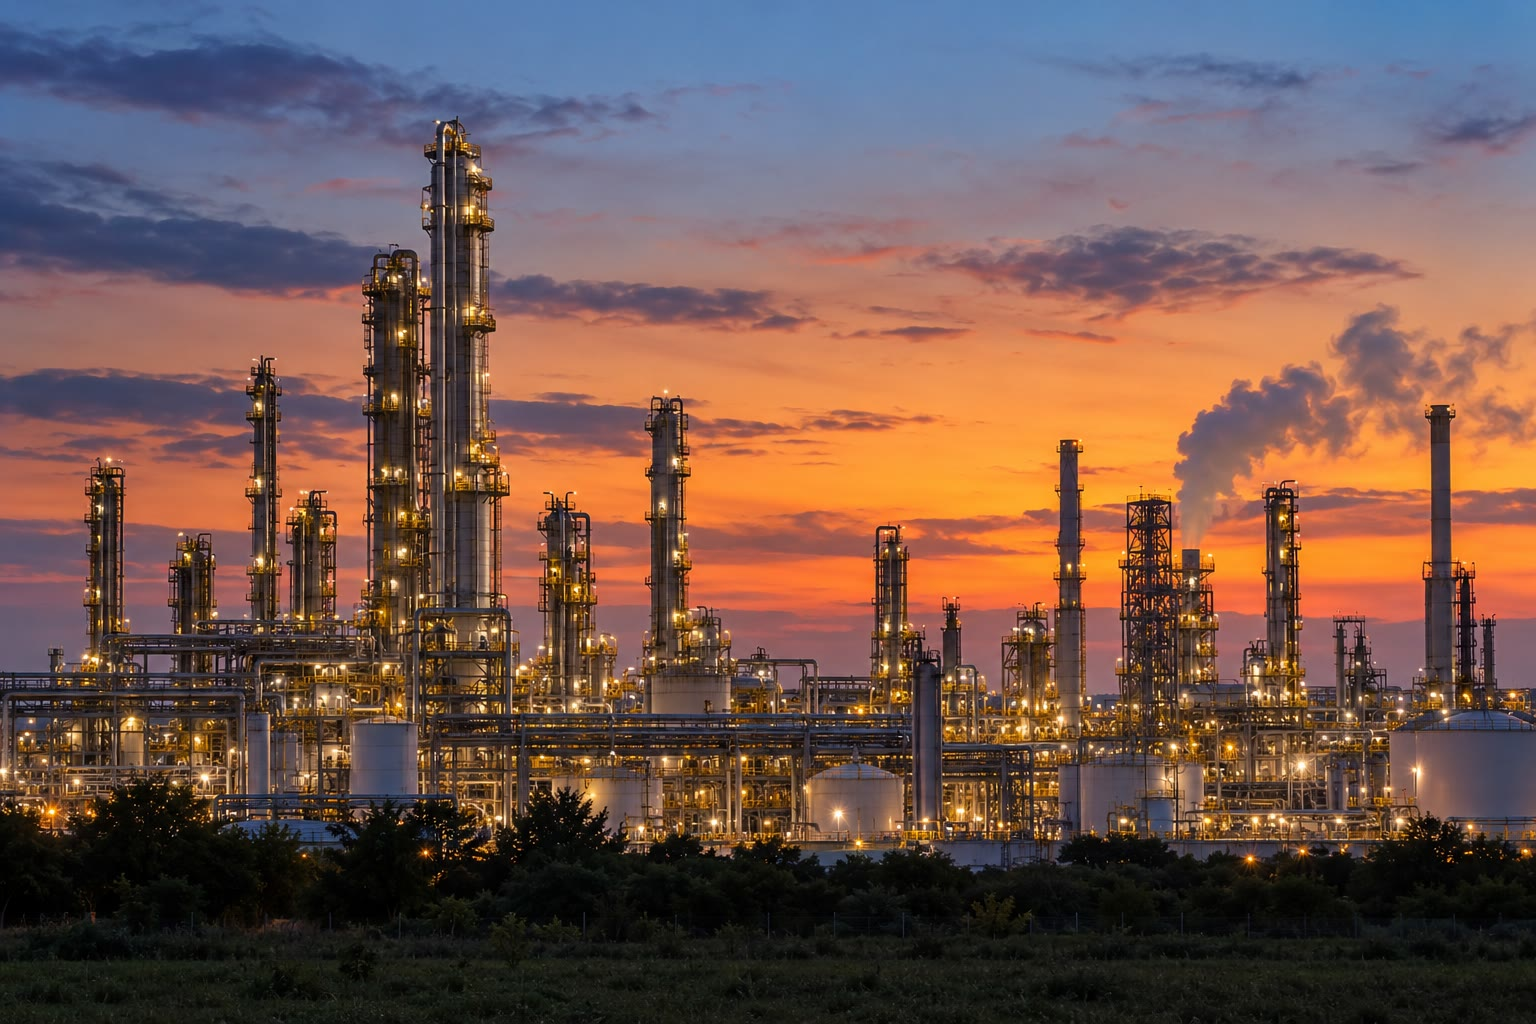
\includegraphics[width=0.6\linewidth]{images/book4/ai/b3-21-chemical-plant.jpg}

{\small Een grote chemische fabriek in de schemering. In een
carbonyleringseenheid is de katalysator een metaalcomplex dat in de
reactievloeistof opgelost is; het grootste deel van de fabriek scheidt
en recycleert.}
\end{omfigure}

\section{Hydrogenering}

\begin{method}[Een katalytische cyclus lezen]\label{met:b3:homogeneous-catalysis:read-cycle}
\begin{enumerate}
  \item Tel bij elke species de valentie-elektronen en geef de
        oxidatietoestand en de $d^n$-configuratie van het metaal.
  \item Benoem elke stap (verlies of opname van een ligand, oxidatieve
        additie, insertie, eliminatie) en controleer dat de tellingen
        veranderen zoals de stap vereist
        (oxidatieve additie: $+2$ in oxidatietoestand en in elektronentelling).
  \item Bepaal de rusttoestand (de species die zich ophoopt) en de
        snelheidsbepalende stap; de snelheidswet volgt uit de
        voorevenwichten ertussen.
\end{enumerate}
\end{method}

\begin{omfigure}
\begin{tikzpicture}[font=\small, >=Stealth]
  \node (a) at (90:2.3) {\ce{RhCl(PPh3)2} \ (14, Rh$^{\mathrm I}$)};
  \node (b) at (0:3.0) {\ce{RhClH2(PPh3)2} \ (16, Rh$^{\mathrm{III}}$)};
  \node (c) at (-90:2.3) {\ce{RhClH2(RCH=CH2)(PPh3)2} \ (18)};
  \node (d) at (180:3.1) {\ce{RhClH(CH2CH2R)(PPh3)2} \ (16)};
  \draw[->, thick] (a) to[bend left=22] node[midway, above right, font=\scriptsize] {$+\,\ce{H2}$, oxidatieve additie} (b);
  \draw[->, thick] (b) to[bend left=22] node[midway, below right, font=\scriptsize] {$+$ alkeen} (c);
  \draw[->, thick] (c) to[bend left=22] node[midway, below left, font=\scriptsize] {migratorische insertie} (d);
  \draw[->, thick] (d) to[bend left=22] node[midway, above left, font=\scriptsize, align=right] {reductieve\\ eliminatie: $-$ alkaan} (a);
  \node[anchor=south] (p) at (90:3.4) {\ce{RhCl(PPh3)3} \ (16, prekatalysator)};
  \draw[<->, black!50] (p) -- (a) node[midway, right, font=\scriptsize] {$\mp\,\ce{PPh3}$};
\end{tikzpicture}

{\small Een vereenvoudigde cyclus van de hydrogenering van alkenen met de
katalysator van Wilkinson (aantal valentie-elektronen tussen haakjes).
Het verlies van een fosfine maakt een plaats vrij; de cyclus neemt
waterstof op, bindt het alkeen, voegt het in in een binding Rh--H en
elimineert het alkaan.}
\end{omfigure}

\begin{proposition}[Kinetiek van Wilkinson]\label{prop:b3:homogeneous-catalysis:wilkinson-rate}
Als $\ce{RhClL3} \rightleftharpoons \ce{RhClL2} + \mathrm L$ ($K_1$) en $\ce{RhClL2} + \ce{H2} \rightleftharpoons \ce{RhClH2L2}$ ($K_2$) snelle
evenwichten zijn en de reactie van het dihydride met het alkeen (snelheidsconstante $k$)
snelheidsbepalend is, is
\[
  v = \frac{kK_1K_2[\mathrm{Rh}]_{\mathrm{tot}}[\ce{H2}][\text{alkeen}]}{[\mathrm L] + K_1 + K_1K_2[\ce{H2}]},
\]
wat verzadigt in waterstof en geremd wordt door toegevoegd fosfine L.
\end{proposition}

\begin{proof}
$[\ce{RhClL2}] = K_1[\ce{RhClL3}]/[\mathrm L]$ en $[\ce{RhClH2L2}] = K_2[\ce{H2}][\ce{RhClL2}]$. Schrijf $[\mathrm{Rh}]_{\mathrm{tot}}$ als de
som van de drie species en los op naar het dihydride: dan is $[\ce{RhClH2L2}] =
K_1K_2[\ce{H2}][\mathrm{Rh}]_{\mathrm{tot}}/([\mathrm L] + K_1 + K_1K_2[\ce{H2}])$; de snelheid is $k$ maal dit en de
alkeenconcentratie.
\end{proof}

De katalysator van Wilkinson hydrogeneert ongehinderde alkenen veel
sneller dan gesubstitueerde en laat carbonylgroepen ongemoeid: de
selectiviteit van een volgepakt metaalcentrum. Chirale difosfines maken
van dezelfde chemie asymmetrische hydrogenering
(\cref{ch:b3:asymmetric-synthesis}).

\section{Carbonyleringsprocessen}

\begin{definition}[Hydroformylering]\label{def:b3:homogeneous-catalysis:hydroformylation}
\emph{Hydroformylering}\index{hydroformylering} is de additie van een
waterstofatoom en een formylgroep (CHO) over een dubbele binding C=C, uit $\ce{H2}$ en CO, waardoor een
alkeen een aldehyde met één koolstofatoom meer wordt. De
\emph{lineair-vertaktverhouding}\index{lineair-vertaktverhouding} is de
verhouding van het onvertakte aldehyde tot het vertakte.
\end{definition}

De eerste processen gebruikten $\ce{HCo(CO)4}$ bij ongeveer 150 tot \qty{180}{\celsius} en zeer hoge
drukken. Rodium met trifenylfosfine werkt rond \qty{100}{\celsius} en bij
veel lagere drukken, en geeft een hogere \omterm{def:b3:homogeneous-catalysis:hydroformylation}{lineair-vertaktverhouding}: de
omvangrijke fosfines begunstigen de insertie die het metaal op het
eindstandige koolstofatoom zet.
Propeen geeft butanal, dat gehydrogeneerd wordt tot butanol of omgezet
in alcoholen voor weekmakers.

\begin{definition}[Carbonylering]\label{def:b3:homogeneous-catalysis:carbonylation}
\emph{Carbonylering}\index{carbonylering} is het invoeren van een
carbonylgroep in een molecuul door reactie met koolstofmonoxide,
gekatalyseerd door een metaalcomplex via de migratorische insertie van
CO.
\end{definition}

De \omterm{def:b3:homogeneous-catalysis:carbonylation}{carbonylering} van methanol tot azijnzuur, $\ce{CH3OH + CO -> CH3COOH}$, verloopt op
rodium (het Monsantoproces) of iridium (het Cativaproces) met methyljodide
als cokatalysator: waterstofjodide zet methanol om in methyljodide, het
metaal voegt CO in in de methylgroep, en het gevormde acetyljodide wordt
gehydrolyseerd, waarbij weer HI vrijkomt.

\begin{omfigure}
\begin{tikzpicture}[font=\small, >=Stealth]
  \node (a) at (90:2.1) {$\ce{[M(CO)2I2]-}$ (16)};
  \node (b) at (0:2.9) {$\ce{[CH3M(CO)2I3]-}$ (18)};
  \node (c) at (-90:2.1) {$\ce{[CH3COM(CO)I3]-}$ (16)};
  \node (d) at (180:2.9) {$\ce{[CH3COM(CO)2I3]-}$ (18)};
  \draw[->, thick] (a) to[bend left=22] node[midway, above right, font=\scriptsize, align=left] {$+\,\ce{CH3I}$\\ oxidatieve additie} (b);
  \draw[->, thick] (b) to[bend left=22] node[midway, below right, font=\scriptsize] {migratorische insertie} (c);
  \draw[->, thick] (c) to[bend left=22] node[midway, below left, font=\scriptsize] {$+$ CO} (d);
  \draw[->, thick] (d) to[bend left=22] node[midway, above left, font=\scriptsize, align=right] {reductieve eliminatie\\ $-\,\ce{CH3COI}$} (a);
  \node[anchor=north, align=center, font=\scriptsize] at (0,-2.55) {$\ce{CH3COI + H2O -> CH3COOH + HI}$, \quad $\ce{CH3OH + HI -> CH3I + H2O}$};
\end{tikzpicture}

{\small De carbonyleringscyclus van methanol voor $\mathrm M = \mathrm{Rh}$ (Monsanto); aantal
valentie-elektronen tussen haakjes, oxidatietoestand van het metaal I
bovenaan, III elders.
Met rodium is de oxidatieve additie van methyljodide snelheidsbepalend.
Met iridium (Cativa) verloopt die veel sneller, is de migratorische
insertie traag, en versnellen
\omterm{def:b3:surfaces-catalysis:catalyst-design}{promotoren} die één jodide van $\ce{[CH3Ir(CO)2I3]-}$ wegnemen de insertie.}
\end{omfigure}

\begin{proposition}[Snelheidswet van het rodiumproces]\label{prop:b3:homogeneous-catalysis:monsanto-rate}
Als de oxidatieve additie van methyljodide aan $\ce{[Rh(CO)2I2]-}$ snelheidsbepalend is en
dit complex de rusttoestand is, is $v = k[\mathrm{Rh}]_{\mathrm{tot}}[\ce{CH3I}]$: van de nulde orde in CO en in
methanol.
\end{proposition}

\begin{proof}
De snelheid is die van de trage stap, $k[\ce{[Rh(CO)2I2]-}][\ce{CH3I}]$, en bijna al het rodium
is in de rusttoestand. CO komt pas na de trage stap binnen, en methanol
regenereert alleen methyljodide, waarvan de stationaire concentratie
bepaald wordt door het jodide dat in de reactor gebracht is en niet door
de methanol.
\end{proof}

Iridium won het in nieuwe fabrieken van rodium om praktische redenen:
zijn complexen blijven in oplossing bij lagere waterconcentraties, wat
energie bespaart bij het drogen van het product, en ze geven minder
bijproducten. De belangrijkste nevenreactie van beide is de
watergasshiftreactie, $\ce{CO + H2O -> CO2 + H2}$, gekatalyseerd door hetzelfde metaal, die
koolstofmonoxide verspilt.

\section{Olefinemetathese}

\begin{definition}[Olefinemetathese]\label{def:b3:homogeneous-catalysis:metathesis}
\emph{Olefinemetathese}\index{olefinemetathese} is de uitwisseling van de
alkylideenhelften van twee alkenen, $\mathrm{RCH{=}CHR + R'CH{=}CHR' \rightleftharpoons 2\,RCH{=}CHR'}$, gekatalyseerd door
metaalcarbeencomplexen via een
\emph{metallacyclobutaan}\index{metallacyclobutaan},
een vierledige ring van het metaal en drie koolstofatomen. Haar
synthetische vormen zijn de
\emph{ringsluitende metathese}\index{ringsluitende metathese} (RCM), die
twee alkeenuiteinden van één molecuul tot een ring verbindt onder verlies
van etheen, de
\emph{ringopenende metathesepolymerisatie}\index{ringopenende metathesepolymerisatie}
(ROMP) van gespannen cyclische alkenen, en de
\emph{kruismetathese}\index{kruismetathese} tussen twee verschillende
alkenen.
\end{definition}

\begin{definition}[Mechanisme van Chauvin]\label{def:b3:homogeneous-catalysis:chauvin}
Het \emph{mechanisme van Chauvin}\index{mechanisme van Chauvin} van de
metathese is de
$[2+2]$-cycloadditie van een alkeen aan een metaalcarbeen, $\mathrm{[M]{=}CHR}$, die een
\omterm{def:b3:homogeneous-catalysis:metathesis}{metallacyclobutaan} geeft, gevolgd door de cycloreversie ervan in de andere
richting, die een nieuw alkeen en een nieuw \omterm{def:b3:organometallic-bonding:carbene}{carbeen} vrijzet.
\end{definition}

\begin{omfigure}
\setchemfig{atom sep=2.1em}
\schemestart
\chemfig{M=[:0]CHR}
\+
\chemfig{R'HC=[:0]CHR'}
\arrow{<=>}
\chemfig{M?-[:0]CHR-[:-90]CHR'-[:180]CHR'?}
\arrow{<=>}
\chemfig{M=[:0]CHR'}
\+
\chemfig{RHC=[:0]CHR'}
\schemestop
\par\vspace{10pt}

{\small Het \omterm{def:b3:homogeneous-catalysis:chauvin}{mechanisme van Chauvin}: een metaalcarbeen en een alkeen
combineren tot een \omterm{def:b3:homogeneous-catalysis:metathesis}{metallacyclobutaan}, dat zich in de andere richting
opent tot een nieuw \omterm{def:b3:organometallic-bonding:carbene}{carbeen} en een nieuw alkeen. Elke stap is
omkeerbaar: metathese bereikt een evenwicht, tenzij een product
vertrekt.}
\end{omfigure}

\begin{proposition}[Ringsluitende metathese aandrijven]\label{prop:b3:homogeneous-catalysis:metathesis-equilibrium}
Voor een ringsluiting $\text{dieen} \rightleftharpoons \text{cycloalkeen} + \ce{C2H4}$ drijft het verwijderen van etheen uit de
oplossing de reactie tot volledigheid; de reactie wordt begunstigd door
de entropie van het vrijkomen van een gasmolecuul.
\end{proposition}

\begin{proof}
In evenwicht is $K = [\text{ring}][\ce{C2H4}]/[\text{dieen}]$: als $[\ce{C2H4}]$ laag gehouden wordt door spoelen of
vacuüm, groeit $[\text{ring}]/[\text{dieen}] = K/[\ce{C2H4}]$ onbegrensd. Het aantal moleculen
neemt bij de reactie met één toe, terwijl de gevormde en verbroken
bindingen (telkens een C=C) gelijkaardig zijn: $\Delta_rH^\circ \approx 0$ voor een ongespannen ring en $\Delta_rS^\circ > 0$, dus $K$ is gunstig.
\end{proof}

ROMP van gespannen ringen, zoals norborneen, verloopt om de omgekeerde
reden in de andere richting: het vrijkomen van ringspanning betaalt voor
het verlies aan translatie-entropie.
De rutheniumcarbenen van Robert Grubbs verdragen water, lucht en de
meeste functionele groepen; de molybdeen- en wolfraamalkylidenen van
Richard Schrock zijn actiever en kunnen enantioselectief gemaakt worden.

\section{Kruiskoppeling met palladium}

\begin{definition}[Kruiskoppelingsreacties]\label{def:b3:homogeneous-catalysis:cross-coupling}
Een \emph{kruiskoppelingsreactie}\index{kruiskoppelingsreactie} verbindt
twee verschillende koolstoffragmenten, een organisch halogenide en een
organometaalreagens of een alkeen, op een metaalkatalysator, meestal
palladium. Bij de
\emph{heckreactie}\index{heckreactie} koppelt een aryl- of vinylhalogenide
met een alkeen, wat een gesubstitueerd alkeen geeft; bij de
\emph{Suzuki-Miyaurakoppeling}\index{Suzuki-Miyaurakoppeling} koppelt het
met een organoboorverbinding in aanwezigheid van een base.
\end{definition}

\begin{omfigure}
\begin{tikzpicture}[font=\small, >=Stealth]
  \node (a) at (90:2.0) {$\mathrm{Pd^0L_2}$};
  \node (b) at (0:2.6) {$\mathrm{ArPd^{II}XL_2}$};
  \node (c) at (-90:2.0) {$\mathrm{ArPd^{II}Ar'L_2}$};
  \draw[->, thick] (a) to[bend left=25] node[midway, above right, font=\scriptsize, align=left] {$+\,$ArX\\ oxidatieve additie} (b);
  \draw[->, thick] (b) to[bend left=25] node[midway, below right, font=\scriptsize, align=left] {$+\,\mathrm{Ar'B(OH)_2}$, base\\ transmetallering} (c);
  \draw[->, thick] (c) to[bend left=35] node[midway, left, font=\scriptsize, align=right] {reductieve eliminatie\\ $-\,$Ar--Ar$'$} (a);
\end{tikzpicture}

{\small De cyclus van Suzuki-Miyaura: palladium(0) voegt zich in in de
binding C--X van het arylhalogenide, ontvangt de tweede arylgroep van het
boorzuur dat door de base geactiveerd is, en zet het biaryl vrij door
reductieve eliminatie.}
\end{omfigure}

\begin{method}[Een kruiskoppeling kiezen]\label{met:b3:homogeneous-catalysis:choose-coupling}
\begin{enumerate}
  \item Disconnecteer het doelmolecuul aan de binding C--C die gevormd moet
        worden; de ene partner wordt het
        halogenide (jodide $>$ bromide $>$ triflaat $>$ chloride in reactiviteit), de andere het
        boorzuur (Suzuki-Miyaura), het alkeen (Heck), de organozinkverbinding
        (Negishi) of het eindstandige alkyn met koper(I) (Sonogashira).
  \item Geef de voorkeur aan het partnerpaar waarvan de reagentia stabiel,
        beschikbaar en het minst giftig zijn: boorzuren voor biarylen.
  \item Kies het ligand voor de moeilijkste stap: elektronenrijke,
        omvangrijke fosfines of N-heterocyclische \omterm{def:b3:organometallic-bonding:carbene}{carbenen} versnellen de
        oxidatieve additie van chloriden.
  \item Plan de verwijdering van palladium uit het product tot de lage
        niveaus die in geneesmiddelen toegelaten zijn (scavengerharsen,
        kristallisatie).
\end{enumerate}
\end{method}

\section{Polymerisatiekatalyse}

\begin{definition}[Ziegler-nattakatalyse]\label{def:b3:homogeneous-catalysis:ziegler-natta}
Een \emph{ziegler-nattakatalysator}\index{ziegler-nattakatalysator}
polymeriseert alkenen bij lage druk; hij wordt gemaakt uit een
overgangsmetaalhalogenide, typisch van titaan, en een
alkylaluminiumverbinding. Het
\emph{mechanisme van Cossee-Arlman}\index{mechanisme van Cossee-Arlman}
van de ketengroei is de coördinatie van het alkeen op een vrije plaats
cis ten opzichte van de groeiende alkylketen op het metaal, gevolgd door
zijn migratorische insertie in de binding metaal-koolstof, wat opnieuw
een vrije plaats achterlaat. Een
\emph{single-sitekatalysator}\index{single-sitekatalysator} heeft al zijn
actieve centra identiek, zoals een moleculaire metalloceenkatalysator.
\end{definition}

\begin{omfigure}
\begin{tikzpicture}[font=\small, >=Stealth]
  \begin{scope}[every node/.style={inner sep=1pt}]
  % panel 1: chain and vacant site
  \node (m1) at (0,0) {M};
  \node (p1) at (-0.7,0.55) {P};
  \node (v1) at (0.7,0.55) {$\square$};
  \draw (m1) -- (p1);
  % panel 2: alkene bound side-on at the vacant site
  \node (m2) at (3.6,0) {M};
  \node (p2) at (2.9,0.55) {P};
  \node (c2a) at (4.75,1.25) {\ce{CH2}};
  \node (c2b) at (4.75,0.25) {\ce{CH2}};
  \draw (m2) -- (p2);
  \draw[double, double distance=1.6pt] (c2a) -- (c2b);
  \draw[dashed] (m2) -- (4.55,0.75);
  % panel 3: chain longer by two carbons, vacant site moved
  \node (m3) at (7.7,0) {M};
  \node (v3) at (7.0,0.55) {$\square$};
  \node (c3a) at (8.45,0.55) {\ce{CH2}};
  \node (c3b) at (8.45,1.45) {\ce{CH2}};
  \node (p3) at (7.75,1.95) {P};
  \draw (m3) -- (c3a) -- (c3b) -- (p3);
  \end{scope}
  \draw[->, thick] (1.25,0.35) -- (2.55,0.35) node[midway, above, font=\scriptsize] {$+\,\ce{C2H4}$};
  \draw[->, thick] (5.35,0.35) -- (6.3,0.35) node[midway, above, font=\scriptsize] {insertie};
\end{tikzpicture}
\par\medskip

{\small Het \omterm{def:b3:homogeneous-catalysis:ziegler-natta}{mechanisme van Cossee-Arlman} (P: de groeiende polymeerketen; $\square$: een
vrije plaats). Het alkeen bindt naast de keten en voegt zich in in de binding M--C
via een vierledige overgangstoestand; de keten, twee koolstofatomen
langer, bezet nu de plaats waar het alkeen zat, en de vrije plaats is
verschoven.}
\end{omfigure}

\begin{proposition}[Tacticiteit uit de symmetrie van de katalysator]\label{prop:b3:homogeneous-catalysis:tacticity-symmetry}
Voor een metalloceenkatalysator waarop de keten bij elke insertie
wisselt tussen twee coördinatieplaatsen, geeft een katalysator met symmetrie $C_2$ isotactisch
polypropeen en een katalysator met symmetrie $C_s$ syndiotactisch polypropeen.
\end{proposition}

\begin{proof}[Beargumenteerd]
Het vlak van het propeen dat zich invoegt, wordt gekozen door de chirale
omgeving van de plaats. In een katalysator met symmetrie $C_2$ worden de twee plaatsen verwisseld door de as $C_2$,
die de handigheid behoudt (\cref{ch:b3:point-groups}): beide plaatsen
kiezen hetzelfde vlak, en opeenvolgende methylgroepen hebben dezelfde
configuratie (isotactisch).
In een katalysator met symmetrie $C_s$ zijn de twee plaatsen spiegelbeelden: ze kiezen
tegengestelde vlakken, en de configuraties wisselen af (syndiotactisch).
Een katalysator waarvan de plaatsen achiraal zijn, zoals onoverbrugd $\ce{Cp2ZrCl2}$ met methylaluminoxaan, geeft atactisch
polymeer.
\end{proof}

\begin{proposition}[Verdeling van Schulz-Flory]\label{prop:b3:homogeneous-catalysis:schulz-flory}
Als elke groeiende keten op een \omterm{def:b3:homogeneous-catalysis:ziegler-natta}{single-sitekatalysator} met constante
waarschijnlijkheid $p$ een monomeer toevoegt en anders overgedragen (beëindigd) wordt, is de aantalsfractie van
ketens met $n$ eenheden $x_n = (1 - p)p^{n-1}$, en de dispersiteit $M_w/M_n = 1 + p$ nadert 2 voor lange ketens.
\end{proposition}

\begin{proof}
Een keten van precies $n$ eenheden is $n - 1$ keer gegroeid en één keer gestopt:
waarschijnlijkheid $p^{n-1}(1 - p)$. Dan is $\sum nx_n = 1/(1 - p)$ (aantalgemiddelde), en de
massafracties $w_n = nx_n(1 - p)$ geven het massagemiddelde $\sum nw_n = (1 + p)/(1 - p)$. Hun
verhouding is $1 + p$.
\end{proof}

\begin{omfigure}
\begin{tikzpicture}
\begin{axis}[width=0.7\linewidth, height=5.2cm, xmin=0, xmax=200, ymin=0, ymax=1.05,
  axis lines=left, xlabel={$M$ / \unit{kg.mol^{-1}}}, ylabel={fractie per eenheid (geschaald)},
  tick label style={font=\small}, label style={font=\small},
  legend style={font=\scriptsize, draw=none, at={(0.98,0.98)}, anchor=north east}, legend cell align=left]
\addplot[omDef, line width=1pt] table[x=M_kg, y=x] {figdata/out/bachelor-3-schulz-flory.dat};
\addplot[omThm, line width=1pt] table[x=M_kg, y expr=\thisrow{w}/0.368] {figdata/out/bachelor-3-schulz-flory.dat};
\draw[black!40, dashed] (axis cs:28.05,0) -- (axis cs:28.05,1);
\node[font=\scriptsize, anchor=west] at (axis cs:30,0.5) {$M_n$};
\legend{aantalsfractie, massafractie (geschaald op haar maximum)}
\end{axis}
\end{tikzpicture}

{\small De meest waarschijnlijke molmassaverdeling van een polyetheen
gemaakt op een \omterm{def:b3:homogeneous-catalysis:ziegler-natta}{single-sitekatalysator} (model: gemiddelde
polymerisatiegraad 1000): de aantalsfractie daalt exponentieel, de massafractie heeft een maximum bij $M_n \approx \qty{28}{kg/mol}$; $M_w = 2M_n$. Klassieke
\omterm{def:b3:homogeneous-catalysis:ziegler-natta}{ziegler-nattakatalysatoren}, met meerdere soorten plaatsen, geven bredere
verdelingen.}
\end{omfigure}

\begin{inthelab}[Een suzukikoppeling en haar palladium]
Het arylbromide, het boorzuur (1.2 equivalenten), kaliumcarbonaat en
enkele tienden van een procent van een palladiumfosfinecomplex worden
onder stikstof bij reflux geroerd in een ontgast mengsel van tolueen,
ethanol en water. Na de opwerking wordt het ruwe biaryl geroerd met een
thiolgefunctionaliseerd silica dat palladium bindt, gefiltreerd en
gekristalliseerd; het achtergebleven palladium wordt gemeten met
plasma-massaspectrometrie.
\end{inthelab}

\begin{safety}{\ghs[0.62cm]{GHS02}\ghs[0.62cm]{GHS04}\ghs[0.62cm]{GHS06}\ghs[0.62cm]{GHS08}}
% ledger: ghs4:MeI, ghs:CO
Methyljodide: giftig bij inademing en inslikken, schadelijk bij contact
met de huid, verdacht kankerverwekkend, vluchtig; gehanteerd in een
zuurkast. Koolstofmonoxide: zeer licht ontvlambaar, giftig bij
inademing, kan het ongeboren kind schaden, reukloos; gebruikt met vaste
detectoren en alarmen.
\end{safety}

\begin{history}[Ziegler, Natta en de metathese]
Karl Ziegler ontdekte in 1953 dat titaanchloride en
alkylaluminiumverbindingen etheen bij atmosferische druk polymeriseren,
en Giulio Natta in 1954 dat zulke katalysatoren stereoregelmatig
polypropeen maken; ze deelden de Nobelprijs voor de Scheikunde van 1963.
Yves Chauvin stelde in 1971 het metallacyclobutaanmechanisme van de
metathese voor; met Robert Grubbs en Richard Schrock, die goed
gedefinieerde metathesekatalysatoren maakten, ontving hij de Nobelprijs
voor de Scheikunde van 2005.
\end{history}

\section{Oefeningen}

\begin{exercise}[$\star$]\label{exo:b3:homogeneous-catalysis:1}
Geef het aantal valentie-elektronen en de oxidatietoestand van rodium bij
elke stap van de cyclus van Wilkinson in de figuur.
\end{exercise}

\begin{exercise}[$\star$]\label{exo:b3:homogeneous-catalysis:2}
Benoem de twee aldehyden die gevormd worden bij de \omterm{def:b3:homogeneous-catalysis:hydroformylation}{hydroformylering} van
propeen. Welk is het onvertakte?
\end{exercise}

\begin{exercise}[$\star$]\label{exo:b3:homogeneous-catalysis:3}
Diethyldiallylmalonaat, $\ce{(CH2=CHCH2)2C(CO2Et)2}$, ondergaat \omterm{def:b3:homogeneous-catalysis:metathesis}{ringsluitende metathese}.
Geef het product en de grootte van zijn ring.
\end{exercise}

\begin{exercise}[$\star$]\label{exo:b3:homogeneous-catalysis:4}
Geef het product van de \omterm{def:b3:homogeneous-catalysis:cross-coupling}{heckreactie} van joodbenzeen met methylacrylaat,
en zijn configuratie.
\end{exercise}

\begin{exercise}[$\star\star$]\label{exo:b3:homogeneous-catalysis:5}
Leid uit de cyclus van het rodiumproces de snelheidswet af, en leg uit
waarom de omzetting van methanol de snelheid niet verandert tot ze bijna
volledig is.
\end{exercise}

\begin{exercise}[$\star\star$]\label{exo:b3:homogeneous-catalysis:6}
Stel twee disconnecties volgens Suzuki-Miyaura voor van
4-methylbifenyl en kies er één.
\end{exercise}

\begin{exercise}[$\star\star$]\label{exo:b3:homogeneous-catalysis:7}
Voorspel de tacticiteit van polypropeen gemaakt met een overbrugde
bis(indenyl)zirkoniumkatalysator met symmetrie $C_2$, met een katalysator met symmetrie $C_s$, en met onoverbrugd $\ce{Cp2ZrCl2}$.
\end{exercise}

\begin{exercise}[$\star\star$]\label{exo:b3:homogeneous-catalysis:8}
Met \qty{0.10}{mol\%} katalysator bereikt een hydrogenering 98\,\% omzetting in \qty{2.0}{h}.
Bereken het turnovergetal en de gemiddelde turnoverfrequentie.
\end{exercise}

\begin{exercise}[$\star\star$]\label{exo:b3:homogeneous-catalysis:9}
Teken de herhalingseenheid van het polymeer gemaakt door ringopenende
metathese van norborneen, en leg uit waarom de reactie volledig
verloopt.
\end{exercise}

\begin{exercise}[$\star\star\star$]\label{exo:b3:homogeneous-catalysis:10}
Een \omterm{def:b3:homogeneous-catalysis:ziegler-natta}{single-sitekatalysator} geeft ketens met $p = 0.9995$. Bereken de
aantalgemiddelde polymerisatiegraad en de dispersiteit. Waarom is een
ziegler-nattapolymeer
breder?
\end{exercise}

\begin{exercise}[$\star\star\star$]\label{exo:b3:homogeneous-catalysis:11}
Toon met de snelheidswet van Wilkinson aan dat de snelheid van de eerste orde in $\ce{H2}$ is bij lage druk
en er bij hoge druk onafhankelijk van is, en dat het toevoegen van
fosfine de reactie vertraagt.
\end{exercise}

\begin{exercise}[$\star\star\star$]\label{exo:b3:homogeneous-catalysis:12}
Leg uit waarom omvangrijke fosfines de \omterm{def:b3:homogeneous-catalysis:hydroformylation}{lineair-vertaktverhouding} bij de
\omterm{def:b3:homogeneous-catalysis:hydroformylation}{hydroformylering} met rodium verhogen, en waarom een hoge verhouding
belangrijk is voor de weekmakeralcoholen die uit de aldehyden gemaakt
worden.
\end{exercise}

\section{Probleem: van methanol tot azijn}

\begin{problem}[{Weekendprobleem --- van methanol tot azijn op een iridiumcyclus:
de tellingen en stappen van de cyclus, de snelheidsbepalende stap en de
promotoren, de turnoverfrequentie van een fabriek, en het
koolstofmonoxide dat aan de watergasshiftreactie verloren gaat}]
\label{pb:b3:homogeneous-catalysis:1}
% ledger: aw:Ir, aw:C, aw:H, aw:O
Een azijnzuurfabriek (gegevens van het probleem) produceert $\qty{5.0e5}{t}$ azijnzuur per jaar
in \qty{8000}{h} bedrijf, met \qty{200}{m^3} reactievloeistof die \qty{5.0}{mmol/L}
iridium bevat. Haar selectiviteit op koolstofmonoxide is 94\,\%: de rest
wordt omgezet door de watergasshiftreactie.

\medskip\noindent\textbf{Deel I --- De cyclus.}
\begin{enumerate}
  \item Tel de elektronen van $\ce{[Ir(CO)2I2]-}$ en geef de oxidatietoestand.
  \item Oxidatieve additie van $\ce{CH3I}$: product, telling, oxidatietoestand?
  \item Verlies van jodide en opname van CO: welk neutraal complex
        ontstaat?
  \item Migratorische insertie: product en telling?
  \item Opname van jodide, daarna reductieve eliminatie van acetyljodide:
        wat wordt geregenereerd?
  \item Schrijf de twee organische stappen op die de cyclus sluiten met
        water en methanol.
  \item Schrijf de totaalreactie op.
\end{enumerate}

\medskip\noindent\textbf{Deel II --- Kinetiek.}
\begin{enumerate}[resume]
  \item Welke stap is snelheidsbepalend met iridium, en hoe verschilt dat
        van rodium?
  \item Hoe versnellen \omterm{def:b3:surfaces-catalysis:catalyst-design}{promotoren} die jodide wegvangen de cyclus?
  \item Welke afhankelijkheid van de jodideconcentratie voorspelt dit?
  \item Waarom is de snelheid onafhankelijk van de methanolconcentratie?
\end{enumerate}

\medskip\noindent\textbf{Deel III --- De fabriek.}
\begin{enumerate}[resume]
  \item Bereken de hoeveelheid azijnzuur die per jaar gemaakt wordt.
  \item Bereken de hoeveelheid per uur.
  \item Bereken de hoeveelheid iridium in de reactor, en de massa ervan.
  \item Bereken de turnoverfrequentie.
  \item Bereken het turnovergetal per jaar.
  \item Bereken de ruimte-tijdopbrengst in kilogram per kubieke meter per
        uur.
\end{enumerate}

\medskip\noindent\textbf{Deel IV --- De watergasshiftreactie.}
\begin{enumerate}[resume]
  \item Schrijf de watergasshiftreactie op.
  \item Bereken het verbruikte CO per mol azijnzuur.
  \item Bereken het gevormde \ce{CO2} per mol azijnzuur.
  \item Bereken de massa \ce{CO2} die per ton azijnzuur uitgestoten wordt.
  \item Waarom helpt werken bij een lagere waterconcentratie, en wat
        begrenst dat?
  \item Welk ander product maakt de shiftreactie, en waarom is het een
        probleem in de reactor?
  \item Formuleer het resultaat: de turnoverfrequentie van de
        iridiumkatalysator.
\end{enumerate}
\end{problem}
